%//==============================--@--==============================//%
\subsection[1.1 Conceitos fundamentais]{\hspace*{0.075 em}\raisebox{0.2 em}{$\pmb{\drsh}$}  Conceitos fundamentais}
\label{subsec:conceitos-fundamentais}

%//==============================--@--==============================//%
\subsubsection[1.1.1 Redes de Computadores]{$\pmb{\rightarrow}$ Redes de Computadores}

Uma rede de computadores pode ser vista como um grupo de sistemas de computação conectados por meio de canais de comunicação em prole da comunicação e partilha de recursos de uma larga gama de utilizadores.

\vspace{-0.5em}
\begin{enumerate}
    \item \textbf{Sistemas terminais} (\textit{end systems or hosts})---e.g., PCs, servidores, quintas de servidores (server farms), telemóveis, laptops, frigoríficos, termostatos, etc.
    \item \textbf{Canal de comunicação} (\textit{peer-to-peer}, difusão)---abstração de comunicação cons- truida sobre um meio físico ou wireless: fios de cobre (e.g., RJ11, RJ45), cabos coaxiais (opção bastante isolada eletromagneticamente), fibra ótica (alta velocidade, opção imune a interferência eletromagnética), rádio nas suas múltiplas variantes...
    \item A interligação supramencionada é efetuada via \textbf{comutadores}, que transitam informação entre canais adjacentes.
    \item Exemplos de \textbf{serviços} de comunicação e partilha de recursos: encaminhamento de dados, garantia de entrega dos dados, autenticação, conversão entre nomes e endereços, etc.
\end{enumerate}

%//==============================--@--==============================//%
\vspace{-2em}
\subsubsection[1.1.2 Internet]{$\pmb{\rightarrow}$ Internet}

A \textit{Internet} é uma "rede de redes", global e hierarquizada, que providencia uma variedade de informação e serviços de comunicação (e.g., \textbf{aplicações distribuidas}) através da \underline{interconexão de redes} que fazem uso de \underline{protocolos} (de comunicação \textbf{standardizados}: abertos, sancionados por uma entidade competente (IETF), mas de adesão voluntária).

\begin{figure}[H]
    \centering
    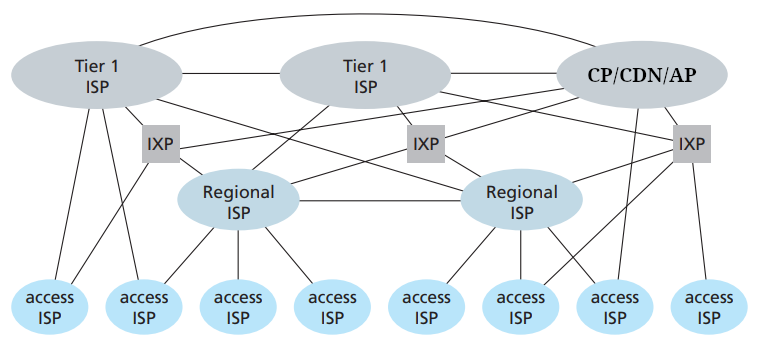
\includegraphics[width = 0.9\linewidth]{img/1/internet-ISP-interconnection.png}
    \caption{Interconexão de ISPs. ``In summary, today’s Internet--—a network of networks—--is complex, consisting of a dozen or so tier-1 ISPs and hundreds of thousands of lower-tier ISPs. The ISPs are diverse in their coverage, with some spanning multiple continents and oceans, and others limited to narrow geographic regions. The lower-tier ISPs connect to the higher-tier ISPs, and the higher-tier ISPs interconnect with one another $[$\textit{peering}, i.e., conectam as suas redes (settlement-free) de forma a que o tráfego comum passe pela conexão direta invés de por um ISP \textit{upstream}$]$.''\cite{Kurose2017}}
    \label{fig:internet}
\end{figure}

\vspace{-2em}
\begin{center}
    \scalebox{0.9}{%
    $$
        \text{CP – Content Provider} \quad \text{CDN – Content Distribution Network} \quad \text{AP – Application Provider}
    $$
    }
\end{center}

\vspace{-0.5em}
\noindent \textbf{Nota:} IXPs {\small(Internet Exchange Points)} são "pontos de encontro" para ISPs fornecidos por \textit{third-parties} que dispõem de infraestruturas independentes com os seus próprios \textbf{comutadores}.
%//==============================--@--==============================//%
\clearpage
\paragraph[1.1.2.1 Protocolos]{$\pmb{\star}$ Protocolos}\mbox{}\\[4pt]
Consideremos agora outra \textit{buzzword} importante em Redes de Computadores: \textit{protocolo}.

\vspace{-2.25em}
\begin{figure}[H] 
    \begin{subfigure}[b]{0.5\linewidth}
        \centering
        \resizebox{\columnwidth}{!}{
            \drawframe{no}
            \setmsckeyword{} %removes msc keyword from the title
            \begin{msc}[
                  normal values,
                  /msc/level height=0.6cm,
                  /msc/label distance=0.5ex,
                  /msc/first level height=0.6cm,
                  /msc/last level height=0.6cm
                ]{}
                \setlength{\instwidth}{2\mscunit} 
                \setlength{\instdist}{2\mscunit} %message width
                
                \declinst{prover}{}{\textbf{Human 1}}
                \declinst{verifier}{}{\textbf{Human 2}}
                \mess{Hi!}{prover}{verifier}
                \nextlevel[2]
                \mess{Hi!}{verifier}{prover}
                \nextlevel[2]
                \mess{Got time?}{prover}{verifier}
                \nextlevel[2]
                \mess{2:00 PM}{verifier}{prover}
            \end{msc}
        }
        \caption{Protocolo "humano".}
        \label{subfig:protocol-example1}
    \end{subfigure}%% 
    \begin{subfigure}[b]{0.5\linewidth}
        \centering
        \resizebox{\columnwidth}{!}{
            \drawframe{no}
            \setmsckeyword{} %removes msc keyword from the title
            \begin{msc}[
                  normal values,
                  /msc/level height=0.6cm,
                  /msc/label distance=0.5ex,
                  /msc/first level height=0.6cm,
                  /msc/last level height=0.6cm
                ]{}
                \setlength{\instwidth}{2\mscunit} 
                \setlength{\instdist}{2\mscunit} %message width
                
                \declinst{prover}{}{\textbf{Client}}
                \declinst{verifier}{}{\textbf{Server}}
                \mess{\footnotesize TCP connection request}{prover}{verifier}
                \nextlevel[2]
                \mess{\footnotesize TCP connection reply}{verifier}{prover}
                \nextlevel[2]
                \mess{\texttt{GET} $\left< \texttt{URL} \right>$}{prover}{verifier}
                \nextlevel[2]
                \mess{$\left< \texttt{file} \right>$}{verifier}{prover}
            \end{msc}
        }
        \caption{Protocolo de rede de computador\protect\footnotemark[1].}
        \label{subfig:protocol-example2}
    \end{subfigure}%% 
    \label{fig:exemplos-protocolos}
    \caption{Exemplos genéricos de protocolos.}
\end{figure}

\vspace{-1em}
\begin{theo}[\underline{Protocolo}]{def:protocolo}\label{def:protocolo}
    ``A \textbf{protocol} defines the format and the order of messages exchanged between two or more communicating entities, as well as the actions taken on the transmission and/or receipt of a message or other event.''\cite{Kurose2017}
\end{theo}

\noindent \textbf{Nota (no contexto computacional):} ``A \textit{protocol} is an agreement about the packets exchanged by communicating programs and what they mean. A protocol tells how packets are structured---for example, where the destination information is located in the packet and how big it is---as well as how the information is to be interpreted.''\cite{Donahoo-Kenneth2002}

\footnotetext[1]{%
    São exemplos de protocolos: TCP, UDP, HTTP/HTTPS; que veremos mais adiante.
}
%//==============================--@--==============================//%
\subsubsection[1.1.3 Breve História das Redes de Computadores e da Internet]{$\pmb{\rightarrow}$ Breve História das Redes de Computadores e da Internet}

\begin{enumerate}[noitemsep, nolistsep] \small
    \item[\textbf{1940:}] Máquina de Turing, primeira noção de um dispositivo computacional com comunicação.
    
    \item[\textbf{1960:}] Mainframes começam a ser utilizadas em universidades e instituições militares para partilhar recursos e comunicar entre si.
    
    \item[\textbf{1969:}] ARPANET, primeira rede de computadores, desenvolvida pelo Departamento de Defesa dos Estados Unidos com o objetivo de conectar instituições de pesquisa.

    \item[\textbf{1972:}] Ray Tomlinson cria o primeiro programa de correio eletrónico, expandindo as funcionalidades da ARPANET além da simples troca de arquivos.
    
    \item[\textbf{1974:}] Vint Cerf e Robert Kahn apresentam o protocolo TCP (Transmission Control Protocol), base para a comunicação na Internet.
    
    \item[\textbf{1983:}] A ARPANET adota o protocolo TCP/IP, sedimentando as bases para a Internet moderna e interconexão global de redes.
        
    \item[\textbf{1989:}] Tim Berners-Lee, no CERN, propõe a World Wide Web, um sistema global de documentos interligados por hiperligações e acessíveis pela Internet.
    
    \item[\textbf{1990:}] ARPANET é oficialmente desativada, dando lugar à Internet atual.
    
    \item[\textbf{1993:}] Mosaic, primeiro navegador gráfico da WWW, desenvolvido por Marc Andreessen e Eric Bina, populariza a Internet e atrai um público mais amplo.
    
    \item[\textbf{1994:}] O protocolo HTTP é desenvolvido por Tim Berners-Lee, facilitando a troca de informações na World Wide Web.
\end{enumerate}

\hfil \textbf{\vdots}

%//==============================--@--==============================//%